%15 min preso!
\documentclass[xcolor=table,aspectratio=169,fleqn]{beamer}
\usepackage{beamerthemesplit}
\usepackage{appendixnumberbeamer}
\usepackage{wrapfig}
\usetheme{SPbGU}
\usepackage{pdfpages}
\usepackage{amsmath}
\usepackage{mathtools}
\usepackage{cmap}
\usepackage[T2A]{fontenc}
\usepackage[utf8]{inputenc}
\usepackage[english]{babel}
\usepackage{indentfirst}
\usepackage{newtxmath}
\usepackage{tikz}
\usepackage{multirow}
\usepackage[noend]{algpseudocode}
\usepackage{algorithm}
\usepackage{algorithmicx}
\usepackage{fancyvrb}
\usepackage{hyperref}
\usepackage{nicematrix}
\definecolor{links}{HTML}{2A1B81}
\hypersetup{colorlinks,linkcolor=,urlcolor=links}
\usetikzlibrary{calc}
\usetikzlibrary{shapes, backgrounds}
\usetikzlibrary{arrows,automata}
\usetikzlibrary{positioning}
\usetikzlibrary{fit}
\usetikzlibrary{shapes.callouts}
\usetikzlibrary{shapes.misc}
\usepackage{xparse}
\usepackage{fontawesome}

\usepackage{etoolbox,refcount}
\usepackage{multicol}

\usepackage{tabularx}
\newcolumntype{Y}{>{\raggedleft\arraybackslash}X}
\setbeamertemplate{itemize item}[circle]
\setbeamertemplate{enumerate item}[circle]


\renewcommand{\thealgorithm}{}

\newtheorem{mytheorem}{Theorem}
\renewcommand{\thealgorithm}{}

\newcommand{\tikzmark}[1]{\tikz[overlay,remember picture] \node (#1) {};}
\def\Put(#1,#2)#3{\leavevmode\makebox(0,0){\put(#1,#2){#3}}}

\newcommand{\ltz}{$< 1$}

\tikzset{
    state/.style={
           rectangle,
           rounded corners,
           draw=black, very thick,
           minimum height=1.5em,
           inner sep=2pt,
           text centered,
           },
}

\tikzset{
    invisible/.style={opacity=0,text opacity=0},
    visible on/.style={alt=#1{}{invisible}},
    alt/.code args={<#1>#2#3}{%
      \alt<#1>{\pgfkeysalso{#2}}{\pgfkeysalso{#3}} % \pgfkeysalso doesn't change the path
    },
}

\tikzset{cross/.style={cross out, draw=black, minimum size=2*(#1-\pgflinewidth), inner sep=0pt, outer sep=0pt, ultra thick},
%default radius will be 1pt. 
cross/.default={1pt}}

\NewDocumentCommand{\mycallout}{r<> O{opacity=0.8,text opacity=1} m m m}{%
\tikz[remember picture, overlay]\node[align=center, fill=cyan!20, text width=#5cm,
#2,visible on=<#1>, rounded corners,
draw,rectangle callout,anchor=pointer,callout relative pointer={(290:0.5cm)}]
at (#3) {#4};
}

\NewDocumentCommand{\mycalloutR}{r<> O{opacity=0.8,text opacity=1} m m m}{%
\tikz[remember picture, overlay]\node[align=center, fill=cyan!20, text width=#5cm,
#2,visible on=<#1>, rounded corners,
draw,rectangle callout,anchor=pointer,callout relative pointer={(30:0.8cm)}]
at (#3) {#4};
}

\newcommand\colR{\cellcolor{red!20}}
\newcommand\colB{\cellcolor{blue!20}}
\newcommand\colG{\cellcolor{green!20}}
\newcommand\colO{\cellcolor{orange!20}}
\definecolor{Gray}{gray}{0.8}

%callout relative pointer={(230:0.5cm)}]

\newcounter{countitems}
\newcounter{nextitemizecount}
\newcommand{\setupcountitems}{%
  \stepcounter{nextitemizecount}%
  \setcounter{countitems}{0}%
  \preto\item{\stepcounter{countitems}}%
}
\makeatletter
\newcommand{\computecountitems}{%
  \edef\@currentlabel{\number\c@countitems}%
  \label{countitems@\number\numexpr\value{nextitemizecount}-1\relax}%
}
\newcommand{\nextitemizecount}{%
  \getrefnumber{countitems@\number\c@nextitemizecount}%
}
\newcommand{\previtemizecount}{%
  \getrefnumber{countitems@\number\numexpr\value{nextitemizecount}-1\relax}%
}
\makeatother    
\newenvironment{AutoMultiColItemize}{%
\ifnumcomp{\nextitemizecount}{>}{3}{\begin{multicols}{2}}{}%
\setupcountitems\begin{itemize}}%
{\end{itemize}%
\unskip\computecountitems\ifnumcomp{\previtemizecount}{>}{3}{\end{multicols}}{}}


\beamertemplatenavigationsymbolsempty


\title[На стыке формальных языков и графов]{Анализ графов с использованием формальных языков в качестве ограничений на пути}
\subtitle{Заготовки для докторской диссертации}
\institute[СПбГУ]{
Санкт-Петербургский Государственный Университет
}

\author[Семён Григорьев]{Семён Григорьев}

\date{!!! !!!! 2026}

\begin{document}
{
\begin{frame}[fragile]
  \begin{table}
  \centering  
  \begin{tabularx}{\linewidth}{XcX}
    \hfill
    & 
    & \hfill \includegraphics[height=1.4cm]{pictures/SPbSU_Logo.pdf}
  \end{tabularx}
  \end{table}
  \titlepage
\end{frame}
}


\begin{frame}[fragile]
  \frametitle{Формальные языки и ограничения на пути в графе}
  \begin{minipage}{0.2\textwidth}
    \begin{tikzpicture}[shorten >=1pt,auto]
      \node[state] (q_0)                      {$0$};
      \node[state] (q_1) [above right=of q_0] {$1$};
      \node[state,fill=red!20] (q_2) [right=of q_0]       {$2$};
      \node[state] (q_3) [right=of q_2]       {$3$};
      \path[->]
      (q_0) edge  node {a} (q_1)
      (q_1) edge  node {a} (q_2)
      (q_2) edge  node {a} (q_0)
      (q_2) edge[bend left, above]  node {b} (q_3)
      (q_3) edge[bend left, below]  node {b} (q_2);
    \end{tikzpicture}
  \end{minipage}
  \begin{minipage}{0.75\textwidth}    
    \begin{itemize}
      \item $G = \langle V, E, L \rangle$ --- (ориентированный) граф с метками на рёбрах
      \item Путь $\pi$ задаёт слово: $\omega(_2 \pi_1) = \omega(2 \xrightarrow{a} 0 \xrightarrow{a} 1) = aa$
      \item Ищем пути, задающие слова определённого вида
      \begin{itemize} 
        \item Например, слова вида $a^*b$
      \end{itemize} 
      \item Множество слов --- язык $\mathcal{L}$ над алфавитом $\Sigma$
      \begin{itemize} 
        \item Для удобства будем считать, что $\Sigma \cap L \neq \varnothing$
      \end{itemize} 
    \end{itemize}
  \end{minipage}
  \vfill
  \pause
  \begin{block}{Варианты задач \textbf{\underline{Formal Language Constrained Path Quering} (FLPQ)}}
    Для данного графа $G$, стартовых вершин $V_s \in V$ и финальных вершин $V_f \in V$, языка $\mathcal{L}$ 
    \begin{itemize}
      \pause
      \item Задача достижимости: $R = \{ (u,v) \mid \omega(_u\pi_v) \in \mathcal{L}, u \in V_s, v \in V_f \}$
      \pause
      \item Задача поиска всех путей: $P = \{ \pi \mid \omega(_u\pi_v) \in \mathcal{L}, u \in V_s, v \in V_f \}$
      \pause
      \item Задача поиска одного пути
      \item Задача проверки наличия достижимых пар
    \end{itemize}
  \end{block}

\end{frame}

\begin{frame}
  \frametitle{Задача на стыке областей}
  \begin{minipage}[t]{0.49\textwidth}
    \begin{center}
      \textbf{Теория графов}
    \end{center}
    \begin{itemize}
      \item Классические варианты известных задач
      \begin{itemize}
        \item Достижимость
        \item Поиск путей
        \item Между всем парами вершин
        \item От заданных вершин
        \item \ldots
      \end{itemize}
      \item Способы представления графов
      \item Разновидности графов:
      \begin{itemize}
        \item С циклами
        \item Без циклов
        \item \ldots
      \end{itemize}
    \end{itemize}
  \end{minipage}
  \pause
  \begin{minipage}[t]{0.49\textwidth}
    \begin{center}
      \textbf{Теория формальных языков}
    \end{center}
    \begin{itemize}
      \item Способы задания ограничений
      \begin{itemize}
        \item Автоматы
        \item Грамматики
        \item \ldots
      \end{itemize}
      \item Разрешимость
      \begin{itemize}
        \item Проверка пустоты пересечения языков
        \item Замкнутость относительно пересечения с регулярными языками
        \item \ldots
      \end{itemize}
      \item Представление результата
      \begin{itemize}
        \item Пересечение языков --- язык
        \item Способы задания языков
        \item \ldots
      \end{itemize}
    \end{itemize}
  \end{minipage}
  

\end{frame}

\begin{frame}[fragile]
  \frametitle{Области применения}
  \begin{itemize}
    \item Регулярные языки
    \begin{itemize}
      \item \textbf{\underline{Графовые базы данных}} (Regular Path Queries, RPQ)      
      \begin{itemize}
        \item Поддерживается (частично) в ряде существующих языков запросов (типа Cypher)
      \end{itemize}
    \end{itemize}
    \pause
    \item Контекстно-свободные языки
    \begin{itemize}
      \item \textbf{\underline{Статический анализ кода}} (Context-Free Language Reachability, CFL-r)
      \begin{itemize}
        \item Анализ потока данных (межпроцедурный анализ указателей), разрешение имён, унификация, \ldots
      \end{itemize}
      \item Графовые базы данных (Context-Free Path Querying, CFPQ)
      \begin{itemize}
        \item Биоинформатика, анализ происхождения данных, анализ иерархий (в RDF), \ldots
      \end{itemize}
    \end{itemize}
    \pause
    \item За пределами контекстно-свободных языков
    \begin{itemize}
      \item Многокомпонентные контекстно-свободные (MCFL): статический анализ кода
      \item Линейные конъюнктивные (Linear Conjunctive): статический анализ кода
    \end{itemize}
  \end{itemize}
\end{frame}

\begin{frame}[fragile]
  \frametitle{Запросы с ограничениями в виде регулярных языков}
  \begin{itemize}
    \item Хорошо изучены
      \begin{itemize}
          \item Впервые введены в работе \href{https://dl.acm.org/doi/10.5555/88830.88850}{A. O. Mendelzon and P. T. Wood. 1989. Finding regular simple paths in graph databases.}
          \item Большое количество прикладных и теоретических работ
      \end{itemize}
    \pause
    \item Часть стандартов ISO языков запросов
      \begin{itemize}
        \item ISO/IEC 9075-16:2023 Information technology --- Database languages --- SQL Part 16: \underline{\textbf{Property Graph Queries (SQL/PGQ)}}
        \item ISO/IEC 39075:2024 Information technology --- Database languages --- \underline{\textbf{GQL}}
      \end{itemize}
    \pause
    \item[\faExclamation] Проблемы с производительностью
      \begin{itemize}
        \item \href{https://dl.acm.org/doi/10.5555/3307192}{Angela Bonifati, George Fletcher, Hannes Voigt, and Nikolay Yakovets. 2018. Querying Graphs}
        \item \href{https://dl.acm.org/doi/abs/10.1007/s00778-023-00811-2}{Diego Arroyuelo, et al. 2023. Optimizing RPQs over a compact graph representation}
    \end{itemize}
  \end{itemize}
\end{frame}

\begin{frame}[fragile]
  \frametitle{Запросы с ограничениями в виде контестно-свободных языков}
  \begin{itemize} 
      \item Активно изучаются
      \begin{itemize}
        \item Родоначальники: Томас Репс и Михалис Яннакакис
        \begin{itemize}
          \item \href{https://dl.acm.org/doi/10.5555/271338.271343}{Thomas Reps. 1997. Program analysis via graph reachability}
          \item \href{https://dl.acm.org/doi/10.1145/298514.298576}{Mihalis Yannakakis. 1990. Graph-theoretic methods in database theory}
        \end{itemize}
        \item Большое количество прикладных и теоретических работ
        \item Известные открытые вопросы
        \begin{itemize}
          \item Существование истинно субкубического алгоритма для задачи достижимости
        \end{itemize}
      \end{itemize}
      \pause
      \item Существуют инструменты (академические прототипы) анализа кода на основе CFL-r      
      \begin{itemize}        
        \item \textsc{Pocr}, \textsc{Pearl}, \textsc{Gaspan}, \textsc{Gigascale}, \ldots        
      \end{itemize}      
      \pause
      \item Попытки интегрировать в графовые базы данных
      \begin{itemize}
        \item \href{https://github.com/thobe/openCypher/blob/rpq/cip/1.accepted/CIP2017-02-06-Path-Patterns.adoc}{Предложение о расширении Cypher}
        \item \href{https://openproceedings.org/2021/conf/edbt/p48.pdf}{Arseniy Terekhov et al. 2021. Multiple-Source Context-Free Path Querying in Terms of Linear Algebra}
      \end{itemize} 
      \pause
      \item[\faExclamation] Проблемы с производительностью
      \begin{itemize}
          \item \href{https://dl.acm.org/doi/10.1145/3335783.3335791}{Jochem Kuijpers, George Fletcher, Nikolay Yakovets, and Tobias Lindaaker. 2019. An Experimental Study of Context-Free Path Query Evaluation Methods}
          \item \href{https://dl.acm.org/doi/10.1109/TSE.2024.3437684}{Chenghang Shi, et al. 2024. Pearl: A Multi-Derivation Approach to Efficient CFL-Reachability Solving}
      \end{itemize}
  \end{itemize}
\end{frame}

\begin{frame}[fragile]
  \frametitle{Более широкие классы языков в качесвтве огарничений на пути}
  \begin{itemize}
    \item Перспективны
    \begin{itemize}
      \item Позволяют улучшить <<точность>> некоторых видов анализа кода
    \end{itemize}
  \end{itemize}
  \pause
  \vfill 
  \begin{itemize}
  \item[\faExclamation] Изучены слабо
    \begin{itemize}
      \item \href{https://dl.acm.org/doi/10.1145/3093333.3009848}{Qirun Zhang and Zhendong Su. 2017. Context-sensitive data-dependence analysis via linear conjunctive language reachability}
      \item \href{https://dl.acm.org/doi/10.1145/3704854}{Giovanna Kobus Conrado, Adam Husted Kjelstrøm, Jaco van de Pol, and Andreas Pavlogiannis. 2025. Program Analysis via Multiple Context Free Language Reachability}
      \item \href{https://ntv.ifmo.ru/en/article/21903/reshenie_zadachi_dostizhimosti_v_grafe_s_zadannymi_ogranicheniyami_v_vide_mnogokomponentnoy_kontekstno-svobodnoy_grammatiki_s_ispolzovaniem_umnozheniya_matric.htm}{Epelbaum I.V., Azimov R.Sh., Grigorev S.V. 2023. Multiple context-free path querying by matrix multiplication}    
    \end{itemize}
  \end{itemize}
\end{frame}

\begin{frame}[fragile]
  \frametitle{Высокопроизводительный анализ графов}
 \begin{itemize}
  \item Обобщённая разреженная \textbf{\underline{линейная алгебра}} --- один из перспективных путей к высокопроизводительному анализу графов
  \begin{itemize}
    \item \ <<Естественная>> параллельность --- возможность использовать современное аппаратное обеспечение, в том числе GPGPU
    \item Выразительность --- алгоритмы для достаточно широкий спектра задач выразимы в терминах линейной алгебры
    \begin{itemize}
      \item Транзитивное замыкание, поиск кратчайших путей, обход в ширину
      \item Подсчёт треугольников, построение минимального остовного дерева
      % \item Подсчёт треугольников, \ldots
      \item John S. Baras and George Theodorakopoulos, \href{https://user.eng.umd.edu/~baras/publications/Books/S00245ED1V01Y201001CNT003.pdf}{Path Problems in Networks}, 2010
      
    \end{itemize}
  \end{itemize}
  \pause
  \item \href{https://graphblas.org/}{GraphBLAS API} --- стандарт, декларирующий базовые примитивы линейной алгебры и операции над ними
  \begin{itemize}
    \item Предложена качественная референсная реализация: \href{https://github.com/DrTimothyAldenDavis/GraphBLAS}{SuiteSparse:GraphBLAS}
    \item Разрабатывается библиотеки прикладных алгоритмов \href{https://github.com/GraphBLAS/LAGraph}{LAGraph}
  \end{itemize}
  \pause
  \item[\faExclamation] Не все алгоритмы \textbf{\underline{естественным}} образом выразимы в терминах линейной алгебры
  \item[\faExclamation] Эффективное использование GPGPU --- нетривиальная задача
 \end{itemize}
\end{frame}

\begin{frame}[fragile]
  \frametitle{Обучение}
 \begin{itemize}
  \item Существуют курсы, затрагивающие те или иные аспекты решения задач анализа графов с использованием формальных языков
  \begin{itemize}
    \item Анализ данных, базы данных
    \item Статический анализ кода
  \end{itemize}
  \pause
  \item Курсы затрагивают отдельные аспекты
  \begin{itemize}
    \item Фундаментальные: алгебра, теория графов, \dots
    \item Прикладные: анализ данных, базы данных, построение компиляторов, \dots
  \end{itemize}   
  \vfill
  \pause
  \item[\faExclamation] Целостность картины
  \begin{itemize}
    \item Разные прикладные области используют общий фундамент
  \end{itemize}
  \pause
  \item[\faExclamation] Преподавание фундаментальных дисциплин для инженеров-программистов
  \begin{itemize}
    \item Связь теории и практики
    \item Применимость в конкретных областях
    \begin{itemize}
      \item Теория формальных языков --- синтаксический анализ (языков программирования)
      \item А что, если я не собираюсь заниматься компиляторами?
    \end{itemize}
  \end{itemize}
  
 \end{itemize}
\end{frame}

\begin{frame}[fragile]
  \frametitle{Выводы}
 \begin{itemize}
  \item Анализ графов с использованием формальных языков в качестве ограничений на пути --- активно развивающаяся область, \textbf{\underline{имеющая прикладное значение}}
  \pause
  \item Междисциплинарность: \textbf{\underline{теория графов}}, \textbf{\underline{теория формальных языков}}, \textbf{\underline{линейная алгебра}}, \textbf{\underline{статический анализ кода}}, \textbf{\underline{графовые базы данных}}, \textbf{\underline{параллельные вычисления}}
  \vfill
  \pause
  \item[\faExclamation] Отсутствие системности в исследованиях
  \begin{itemize}
    \item Выстраивание междисциплинарных связей
    \item Переиспользование методов, инструментов, терминологии, \ldots
    \item Сопоставление результатов
  \end{itemize}
  \pause
  \item[\faExclamation] Проблемы с прикладными алгоритмами
  \begin{itemize}
    \item Точечные решения вместо методов решения классов задач
    \item Плохая производительность
    \item Слабая база для экспериментальных исследований
  \end{itemize}
  \pause
  \item[\faExclamation] Отсутствие системности в подготовке специалистов
  \begin{itemize}
    \item Выстраивание междисциплинарных связей
    \item Формирование целостной картины
  \end{itemize}
 \end{itemize}
\end{frame}

\begin{frame}[fragile]
  \frametitle{Цель работы}
  Целью данной работы является создание методологии \underline{анализа графов} с использованием \underline{формальных языков} в качестве \underline{ограничений на пути}
  \begin{itemize}
    \item Нацеленную на получение практически значимых результатов
    \item Предоставляющую гибкий подход к решению задач
    \item Позволяющую формально рассуждать о свойствах объектов (модели, алгоритмы)
  \end{itemize}

\end{frame}


\begin{frame}[fragile]
  \frametitle{Положения, выносимые на защиту}
  \begin{enumerate}[<+->]
    \item Создана методология анализа графов с использованием формальных языков в качестве ограничений на пути, нацеленная на конструирование алгоритмов FLPQ    
    \item Разработаны методы конструирования алгоритмов решения FLPQ
    \begin{itemize} 
      \item Использующих операции линейной алгебры
      \item Основанных на классических алгоритмах синтаксического анализа
    \end{itemize}
    \item Разработаны методические рекомендации по проведению экспериментальных исследований решений FLPQ
    \item Спроектированы и реализованы библиотеки разреженной линейной алгебры, использующие графические ускорители для решения FLPQ
    \item Создан набор данных для экспериментального исследования решений FLPQ
    \item Разработаны, реализованы, интегрированы в пользовательские библиотеки и инструменты алгоритмы решения различных вариантов FLPQ
    \item Разработаны методические рекомендации по выстраиванию междисциплинарных связей, улучшающих понимание областей применения и алгоритмов решения FLPQ
    \item Разработан курс для программных инженеров, выстраивающий изучение основ теории формальных языков вокруг различных вариантов FLPQ
  \end{enumerate}
\end{frame}

\begin{frame}[fragile]
  \begin{overprint}
    \only<1>{
      \begin{center}
        \includegraphics[width=\textwidth]{pictures/Methodology_only.pdf}
      \end{center}
    }
  \onslide<2->{
    \begin{minipage}{0.45\textwidth}
        \includegraphics[width=\textwidth]{pictures/Methodology_only.pdf}
    \end{minipage}
    \begin{minipage}{0.53\textwidth}
        \begin{itemize}
          \item \underline{Объект} --- задачи анализа графов с использованием формальных языков в качестве ограничений на пути
          \item \underline{Предмет} --- алгоритмы решения задач анализа графов с использованием формальных языков в качестве ограничений на пути
        \end{itemize}
    \end{minipage}
    \onslide<3->{
    \begin{itemize}
      \item \underline{Теоретическая обоснованность}: границы применимости, оценки сложности, доказательство корректности
      \item \underline{Универсальность}: возможность построить решатели в стиле SAT или SMT
      \item \underline{Настраиваемость}: класс языков $\longleftrightarrow$ структура графа $\longleftrightarrow$ библиотеки
      %\item \underline{Декларативность} $\Rightarrow$ \underline{Эволюционность}: проще внедрять новые результаты 
      \item \underline{Эволюционность}: использование новых результатов из конкретных областей
      \item \underline{Основные фазы} (цикл)
      \begin{itemize}
        \item Формулировка задачи, моделирование предметной области
        \item Дизайн: построение алгоритма, теоретический анализ
        \item Разработка: реализация алгоритма, оптимизации
        \item Экспериментальное исследование: оценка показателей, сравнительный анализ
      \end{itemize}
    }
    \end{itemize}
  }
  \end{overprint}
\end{frame}


\begin{frame}[fragile]
  \begin{center}
    \begin{overprint}
      \only<1>{\includegraphics[width=\textwidth]{pictures/Methodology_0.pdf}}
      \only<2>{\includegraphics[width=\textwidth]{pictures/Methodology_1.pdf}}
      \only<3>{\includegraphics[width=\textwidth]{pictures/Methodology_2.pdf}}
      \only<4>{\includegraphics[width=\textwidth]{pictures/Methodology_full.pdf}}
    \end{overprint}
  \end{center}
\end{frame}

\begin{frame}[fragile]
  \frametitle{Метод конструирования алгоритмов FLPQ, основанных на линейной алгебре}
   \begin{overprint}
    \only<1>{
      \begin{center}
    \includegraphics[width=\textwidth]{pictures/Method_LinAlg.pdf}
  \end{center}
    }
  \onslide<2->{
    \begin{minipage}{0.45\textwidth}
        \includegraphics[width=\textwidth]{pictures/Method_LinAlg.pdf}
    \end{minipage}
    \begin{minipage}{0.53\textwidth}
        \begin{itemize}
          \item \underline{Основная идея} --- дуализм отношений и линейной алгебры
          \item \underline{Преимущества}
          \begin{itemize}
            \item Автоматически параллельные алгоритмы с высокой реальной производительностью
            \item Инженерная вычислительная сложность хорошо разграничена абстрагирована
          \end{itemize}
        \end{itemize}
    \end{minipage}
    \onslide<3->{
    \begin{itemize}
      \item \underline{Недостатки}
      \begin{itemize}
        \item Нетривиальный переход от прикладных задач к алгебраическим структурам
        \item Сложно эффективно реализовать работу с путями        
      \end{itemize}
      \item \underline{Ограничения}
      \begin{itemize}
        \item Представление графа --- вариации матрицы смежности
        \item Эффективная реализация требует хороших библиотек разреженной линейной алгебры
        \item Нет учёта дополнительных ограничений на пути (простота, гамильтоновость и т.д.)
        \item Нет фокуса на улучшении теоретических оценок
      \end{itemize}
    }
    \end{itemize}
  }
  \end{overprint}
\end{frame}

\begin{frame}[fragile]
  \frametitle{Алгоритмы FLPQ, основанные на линейной алгебре}
  \begin{itemize}
    %\item Получены \textbf{\underline{новые}} алгоритмы анализа графов с использованием следующих классов языков в качестве ограничений
    \item \textbf{\underline{Новые}} алгоритмы анализа графов с использованием следующих классов языков
    \begin{itemize}
      \item Регулярные языки (RPQ)
      \item Контекстно-свободные языки (CFPQ)
      \item Булевы и конъюнктивные языки
      \item Многокомпонентные контекстно-свободные языки
    \end{itemize}
    \pause
    \item Решаются различные варианты задач FLPQ
    \begin{itemize}
      \item Достижимость
      \item Поиск путей
      \item Между всеми парами вершин
      \item От заданного множества вершин
    \end{itemize}
    \pause
    \item Используются разнообразные операции линейной алгебры
    \begin{itemize}
      \item Поэлементные операции над матрицами и векторами
      \item Умножение матриц и матрицы на вектор в различных полукольцах
      \item Произведение Кронекера
    \end{itemize}
    \pause
    \item Сформулированы и доказаны теоремы о корректности полученных алгоритмов
    \item Получены оценки сложности для предложенных алгоритмов
  \end{itemize}
\end{frame}

\begin{frame}[fragile]
  \frametitle{Метод конструирования алгоритмов FLPQ, основанных на классических алгоритмах синтаксического анализа}
  \begin{overprint}
    \only<1>{
      \begin{center}
    \includegraphics[width=\textwidth]{pictures/Method_Parsing.pdf}
  \end{center}
    }
  \onslide<2->{
    \begin{minipage}{0.45\textwidth}
        \includegraphics[width=\textwidth]{pictures/Method_Parsing.pdf}
    \end{minipage}
    \begin{minipage}{0.53\textwidth}
        \begin{itemize}
          \item \underline{Основная идея} --- обобщение \emph{обобщённых} (generalized) алгоритмов анализа
          \begin{itemize}
            \item Добавление конфликта типа <<перенос-перенос>>
          \end{itemize}
          \item \underline{Преимущества}
          \begin{itemize}
            \item Обобщение классических алгоритмов
            \item Результат близок к лесу разбора
            \item Направленность поиска
          \end{itemize}
        \end{itemize}
    \end{minipage}
    \onslide<3->{
    \begin{itemize}
      \item \underline{Недостатки}
      \begin{itemize}
        \item Трудно построить эффективную параллельную версию
        \item Менее эффективны по памяти (чем линейная алгебра)
        \item Сложно абстрагировать нетривиальные структуры данных        
      \end{itemize}
      \item \underline{Ограничения}
      \begin{itemize}        
        \item Нет учёта семантических действий (атрибутных грамматик)
        \item Нет учёта дополнительных ограничений на пути (простота, гамильтоновость и т.д.)
      \end{itemize}
    }
    \end{itemize}
  }
  \end{overprint}
\end{frame}

\begin{frame}[fragile]
  \frametitle{Алгоритмы CFPQ, основанные на классических алгоритмах синтаксического анализа}
  \begin{itemize}
    \item \textbf{\underline{Новые}} алгоритмы анализа графов с использованием контекстно-свободных языков
    \pause
    \item Используются различные методы и алгоритмы синтаксического анализа
    \begin{itemize}
      \item Генеративный на основе обобщённого LR (Generalized LR, GLR)
      \item Генеративный на основе обобщённого LL (Generalized LL, GLL)
      \item Комбинаторы парсеров (Parser combinators)
      \item Комбинаторы грамматик (Grammar combinators)
    \end{itemize}
    \pause
    \item Решаются различные варианты задач FLPQ
    \begin{itemize}
      \item Достижимость
      \item Поиск путей
      \item Между всеми парами вершин
      \item От заданного множества вершин
    \end{itemize}
    \pause
    \item Сформулированы и доказаны теоремы о корректности полученных алгоритмов
    \item Получены оценки сложности для предложенных алгоритмов
  \end{itemize}
\end{frame}

\begin{frame}[fragile]
  \frametitle{Методические рекомендации по проведению экспериментальных исследований решений FLPQ}
  \begin{itemize}
    \item Выбор и подготовка входных данных
    \begin{itemize}
      \item Данные из различных прикладных областей (особенно для универсальных решений)
      \item Форма представления запроса существенно влияет на производительность решения
      \item Правила выбора стартовых вершин зависят от предметной области
      \begin{itemize}
        \item Крайне редко стоит выбирать случайные вершины
      \end{itemize}
    \end{itemize}
    \pause
    \item Какие шаги включать в замеры
    \begin{itemize}
      \item Предподготовка данных: существуют <<неотчуждаемые>> преобразования
      \item Постобработка результата
      \begin{itemize}
        \item Достижимость: матрица смежности $\to$ множество пар вершин
        \item Поиск путей: <<индекс>> путей $\to$ отдельные пути (один, несколько, все)
      \end{itemize}
      \item Построение индексов 
      \begin{itemize}
        \item Сохраняем результат для всех вершин, \textbf{быстро} решаем задачу для конкретных вершин
      \end{itemize}
    \end{itemize}
    \pause
    \item Разрешимость проверки эквивалентности результатов для задачи поиска всех путей
    \begin{itemize}
      \item Проверка эквивалентности конечных автоматов в общем случае \textbf{разрешима}
      \item Проверка эквивалентности КС грамматик в общем случае \textbf{неразрешима}
      \item Проверка эквивалентности MCFG в общем случае \textbf{неразрешима}
    \end{itemize}
  \end{itemize}
\end{frame}

\begin{frame}[fragile]
  \frametitle{Набор данных \href{https://github.com/FormalLanguageConstrainedPathQuerying/CFPQ_Data}{CFPQ\_Data}}
  \begin{itemize}
    \item Для экспериментального исследования алгоритмов FLPQ
    \begin{itemize}
      \item Регулярные языки
      \item Контекстно-свободные языки
      \item[\faGears] Многокомпонентные контекстно-свободные языки
    \end{itemize}
    \pause
    \item Синтетические данные
    \begin{itemize}
      \item Крайние случаи
      \item \ <<Случайные>> графы
    \end{itemize}
    \item Реальные данные из различных областей (граф, запросы, стартовые вершины)
    \begin{itemize}
      \item Статический анализ кода
      \item Семантические сети
      \item[\faGears] Биоинформатика
      \item[\faGears] Анализ происхождения данных
    \end{itemize}
    \pause
    \item Метаданные
    \begin{itemize}
      \item Описание: источник, количество вершин, рёбер, метки рёбер
      \item Контрольные значения: ответы на конкретные запросы
    \end{itemize}
  \end{itemize}
\end{frame}

\begin{frame}[fragile]
  \frametitle{Инженерные решения на основе разработанных алгоритмов}
  \begin{itemize}
    \item Разработаны универсальные решатели
    \begin{itemize}
      \item \href{https://github.com/FormalLanguageConstrainedPathQuerying/UCFS}{UCFS} и \href{https://github.com/gsvgit/CFPQ_GLL}{CFPQ\_GLL}: контекстно-свободные языки, на основе GLL
      \item \href{https://github.com/FormalLanguageConstrainedPathQuerying/CFPQ_PyAlgo}{CFPQ\_PyAlgo}: контекстно-свободные языки, на основе линейной алгебры
    \end{itemize}
    \pause
    \item Интеграция с инструментами статического анализа кода
    \begin{itemize}
      \item[\faGears] С SVF --- инструмент для анализа LLVM IR
      \item[\faGears] С Qilin --- инструмент для анализа Java
    \end{itemize}
    \pause
    \item Интеграция в графовые базы данных
    \begin{itemize}
      \item \textbf{\underline{Первая}} полноценная поддержка запросов с ограничениями в виде КС языков
      \begin{itemize}
        \item От языка запросов (Cypher) до алгоритма выполнения в инфрастуктуре БД (RedisGraph)
      \end{itemize}
      \item \textbf{\underline{Самый высокопроизводительный}} алгоритм запросов с КС ограничениями для Neo4j
    \end{itemize}
    \pause
    \item Часть алгоритмов интегрирована в библиотеку LAGraph\footnote{Коллекция алгоритмов анализа графов на основе линейной алгебры}
    \begin{itemize}
      \item Для регулярных и контекстно-свободных языков
    \end{itemize}
    \pause
    \item Отдельные реализации
    \begin{itemize}
      \item Многокомпонентные контекстно-свободные языки в качестве ограничений
      \item Конъюнктивные и булевы языки в качестве ограничений
    \end{itemize}
  \end{itemize}
\end{frame}

\begin{frame}[fragile]
  \frametitle{Библиотеки разреженной линейной алгебры}
  \begin{itemize}
    \item Спроектированы и реализованы библиотеки разреженной линейной алгебры, использующие возможности GPGPU
    \begin{itemize}
      \item Специализированные для булевой алгебры: CuBool (Nvidia Cuda), Spbla (OpenCL)
      \item Обобщённые: Spla (OpenCL), Brahma.FSharp + GraphBLAS\# (F\# + OpenCL)
    \end{itemize} 
    \pause
    \item Показана применимость разработанных библиотек для решения задач анализа графов
    \begin{itemize}
      \item В том числе, некоторых задач FLPQ
    \end{itemize} 
    \pause
    \item Сформулированы рекомендации и ограничения 
    \begin{itemize}
      \item Выделение булевых операций для улучшения производительности
      \item Баланс между трансфером данных и вычислениями (в контексте FLPQ)
      \item Востребованность операций и их модификаций: Kronecker с маской и фильтрами
      \item Использование возможностей функциональных языков программирования (полукольца, Oрtion для матриц смежности)
    \end{itemize} 
  \end{itemize}
\end{frame}

\begin{frame}[fragile]
  \frametitle{Методические рекомендации по преподаванию}
  \begin{itemize}
    \item Теория формальных языков
    \begin{itemize}
      \item Примеры прикладных областей и конкретных задач
      \item Непосредственное использование теоретических результатов
      \item Свежий взгляд на известные задачи (инкрементальный анализ, неоднозначные грамматики)
    \end{itemize}
    \pause
    \item Теория графов
    \begin{itemize}
      \item Использования и обобщения классических алгоритмов (обход в ширину, транзитивное замыкание)
      \item Использования и обобщения классических структур данных (матрица смежности)
      \item Пример класса задач с требованиями к производительности
    \end{itemize}
    \pause
    \item Алгебра
    \begin{itemize}
      \item Применение операций линейной алгебры и их свойств
      \item Нетривиальные алгебраические структуры (неассоциативные полукольца)
    \end{itemize}
    \pause
    \item Анализ программ, графовые базы данных 
    \begin{itemize}
      \item Теоретическая основа
      \item Прикладные алгоритмы, инструменты
    \end{itemize}
  \end{itemize}
\end{frame}

\begin{frame}[fragile]
  \frametitle{Курс по теории формальных языков}
  \begin{itemize}    
      \item Для инженеров-программистов
      \begin{itemize}
        \item Основной акцент на теории, которая важна на практике
        \item Прикладные алгоритмы, особенности их реализации
        \item Связь с другими прикладными областями
      \end{itemize}
      \item Для каждого класса языков: задача $\to$ теоретическая основа $\to$ алгоритмы
      \item Активное использование знаний, полученных на теоретических курсах
      \begin{itemize}
        \item Алгебра
        \item Дискретная математика, теория графов
      \end{itemize}
      \item Классические задачи с нового ракурса
      \begin{itemize}
        \item Инкрементальный синтаксический анализ $\to$ обработка изменяющихся графов
        \item Параллельный синтаксический анализ $\to$ параллельная обработка графов
        \item Работа с неоднозначными грамматиками $\to$ неоднозначные запросы 
      \end{itemize}
    \end{itemize}
\end{frame}

\begin{frame}[fragile]
  \frametitle{Границы применимости}
  \begin{itemize}
    \item Прикладная направленность: основной фокус на получении алгоритмов, имеющих практическую ценность
    \begin{itemize}
      \item Возможно ли улучшить оценки сложности для задачи или класса задач?
    \end{itemize} 
    \pause
    \item Не обсуждаются частные/крайние случаи 
    \begin{itemize}
      \item Что делать, если известно, что граф --- дерево?
      \item Можно ли улучшить решение, если известно, что язык принадлежит специфичному узкому классу?
    \end{itemize}
    \pause
    \item Не обсуждаются некоторые особенностей прикладных областей 
    \begin{itemize}
      \item Реализуем ли мы статический анализ для IDE или же для компилятора
      \item Разрабатываем мы алгоритм для графовой базы данных с OLAP нагрузкой или же с OLTP
    \end{itemize} 
    \pause
    \item Не обсуждается удобство для прикладного пользователя
    \begin{itemize}
     \item Как естественным образом встраивать рассматриваемые ограничения в язык запросов к графам?
     \item Как должен выглядеть интерфейс унифицированного решателя задач FLPQ?
    \end{itemize}
  \end{itemize}
\end{frame}

\begin{frame}[fragile]
  \frametitle{Результаты}
  \begin{enumerate}
    \item Создана методология анализа графов с использованием формальных языков в качестве ограничений на пути, нацеленная на конструирование алгоритмов FLPQ
    \item Разработаны методы конструирования алгоритмов решения FLPQ
    \begin{itemize} 
      \item Использующие операции линейной алгебры
      \item Основанные на классических алгоритмах синтаксического анализа
    \end{itemize}
    \item Разработаны методические рекомендации по проведению экспериментальных исследований решений FLPQ
    \item Спроектированы и реализованы библиотеки разреженной линейной алгебры, использующие графические ускорители для решения FLPQ
    \item Создан набор данных для экспериментального исследования решений FLPQ
    \item Разработаны, реализованы, интегрированы в пользовательские библиотеки и инструменты алгоритмы решения различных вариантов FLPQ
    \item Разработаны методические рекомендации по выстраиванию междисциплинарных связей, улучшающих понимание областей применения и алгоритмов решения FLPQ
    \item Разработан курс для программных инженеров, выстраивающий изучение основ теории формальных языков вокруг различных вариантов FLPQ
  \end{enumerate}

\end{frame}

\appendix

\begin{frame}[fragile]
  \frametitle{Соответствие паспорту специальности 2.3.5}
  \begin{itemize}
    \item Пункту 1: модели, методы и алгоритмы проектирования, анализа, трансформации, верификации и тестирования программ и программных систем
    \item Пункту 4: интеллектуальные системы машинного обучения, управления базами данных и знаний, инструментальные средства разработки цифровых продуктов
    \item Пункту 8: модели и методы создания программ и программных систем для параллельной и распределенной обработки данных, языки и инструментальные средства параллельного программирования
    \item Пункту 10: оценка качества, стандартизация и сопровождение программных систем
  \end{itemize} 
\end{frame}

\begin{frame}[fragile]
  \frametitle{Основные публикации}
  \begin{enumerate}
    \only<1>{
    \item Epelbaum I.V., Azimov R.Sh., Grigorev S.V. Multiple Context-Free Path Querying by Matrix Multiplication // Научно-технический вестник информационных технологий, механики и оптики. 2023.
    \item Egor Orachev, Maria Karpenko, Pavel Alimov, Semyon Grigorev // SPbLA: The Library of GPGPU-powered Sparse Boolean Linear Algebra Operations. Journal of Open Source Software, 2022
    \item Shemetova, E.N., Grigorev, S.V. // Path Querying on Acyclic Graphs Using Boolean Grammars. Program Comput Soft, 2021
    \item Azimov, R., Grigorev, S. // Path Querying with Conjunctive Grammars by Matrix Multiplication. Program Comput Soft, 2019
    \item Shemetova, E., Okhotin, A., Grigorev, S. // Rational Index of Languages Defined by Grammars with Bounded Dimension of Parse Trees. Theory Comput Syst, 2025    
    }
    \only<2>{
    \setcounter{enumi}{5}
    \item Азимов Р. Ш., Григорьев С. В. Алгоритм поиска всех путей в графе с заданными контекстно-свободными ограничениями с использованием матриц с множествами промежуточных вершин // Научно-технический вестник информационных технологий, механики и оптики, 2021
    \item С. В. Григорьев и др., Инструментальная поддержка встроенных языков в интегрированных средах разработки // Модел. и анализ информ. систем, 2014
    \item С. В. Григорьев и др., PereFlex: инструмент для автоматической оценки восстановления после ошибок в синтаксических анализаторах // Труды Института системного программирования РАН, 2025
    \item \faGears
    \item \faGears
    \item \faGears
    }    
  \end{enumerate} 
\end{frame}


\begin{frame}[fragile]
  \frametitle{Конференции, семинары, гранты}
  \begin{itemize}
    \item Конференции (более 10)
    \begin{itemize}
      \item Анализ данных и базы данных: EDBT-2021, ADBIS-2020, DAMDID-2025
      \item Анализ графов: GRADES-NDA-2018/2019/2020/2021, Grapl-2021, LSGDA-2025
      \item Статический анализ кода: SOAP-2025, SIGPLAN International Symposium on Scala 2018
      \item Иное: SECR-2017, PSI-2015, PaCT-2025, SYRCoSE-2025
    \end{itemize}
    \pause
    \item Семинары
    \begin{itemize}
      \item Семинар кафедры Системного программирования
      \item Data.Meetup: графовые решения. Финтех и телеком
    \end{itemize}
    \pause
    \item Гранты
    \begin{itemize}
      \item Грант РНФ 18-11-00100 <<Логические и алгебраические методы в теории формальных языков>>
      \item Грант РФФИ 19-37-90101 <<Поиск путей с ограничениями в терминах формальных языков>>
      \item Грант СПбГУ 116636233 <<Методы искусственного интеллекта в задачах механики сплошных сред>> 
    \end{itemize}
  \end{itemize} 
\end{frame}

\end{document}
